% ----- CHAPTER 6: REMARKS AND FUTURE WORK ----- %

This dissertation pulls in results from a number of disparate topics related to elliptic curves, with the general approach being ``do just enough to establish results that are sufficient to support the main theorems". As such, many of the bounds and statements obtained of the course of this work are very far from optimal, and the ultimate running time of, say, Algorithm \ref{algo:compute_rank} could be considerably improved if these bounds were tightened. In this section we hope to list (in somewhat random order) the areas where results could be improved upon, and in so doing detail directions for possible future work.

%%%%%%%%%%%%%%%%%%%%%%%%%%%%%%%%%%%%%%%%%%%%%%%%%%%%%%%%
\section{Bounding analytic rank from above in terms of conductor}

To establish a lower bound on the regulator of an elliptic curve in terms of its conductor we require an upper bound on the analytic rank. To this end we invoke Corralaries \ref{cor:logderiv_rank_bound} and \ref{cor:better_an_bound}, stating that maximum analytic rank is bounded by $\frac{1}{2}\log N_E$ plus an explicit constant. \\

However, Corollary \ref{cor:rank_slower_than_log_N} asserts that, contingent on GRH, maximum analytic rank of in fact grows slower than log of the conductor. This result has {\it not} been used directly, mainly because the constant $K(\epsilon)$ has not been made explicit in terms of the $\epsilon$ chosen. This translates to bounding the $c_n$ sum
\begin{equation}
\sum_{n < e^{2\pi \Delta}} c_n \cdot \left(1-\frac{\log n}{2\pi \Delta}\right)
\end{equation}
in terms of the parameter $\Delta$. \\

A natural question to ask, and hopefully answer, is ``can this be done effectively"? Empirically, the $c_n$ sum is seldom more than a handful of units in magnitude; however, the fact that the sum is carried out over prime powers and large amounts of cancellation due to the changing signs of the $c_n$ coefficients means that this term is tricky to control [note that one can readily obtain a naive explicit bound, it is exponential in $\log \Delta$, and thus quite useless from a practical perspective]. \\

Nevertheless, if one could show that the sum grows at most polynomial in $\log \Delta$ (regardless of $E$) and obtain explicit constants, then a direct consequence would be that the lower bound on the regulator of $E$ would go to zero more slowly than any negative power of $N$. \\

%%%%%%%%%%%%%%%%%%%%%%%%%%%%%%%%%%%%%%%%%%%%%%%%%%%%%%%%
\section{The regulator}

Orthogonal to the above, a lower bound on $\Reg_E$ relies on Hindry-Silverman's \cite{HiS-1988} result that, contingent on ABC, minimum point height obeys the bound
\begin{equation}
\hat{h}(P) > 6\times 10^{-11}\cdot \log(D_E)
\end{equation}
where $D_E$ is the discriminant of $E$, and $P$ is any rational point on $E$. This result is in all probability {\it very} far from optimal; we recall that the minimum point height known is $8.9\times 10^{-4}$. An improvement in the lower bound on point height would result in a direct improvement on the constants involved in the lower bound on the regulator. Again, this is a deep topic, so new insight here won't come easily. \\

What is perhaps a bit more tractable is to continue in the same vein as in the beginning of the proof of Theorem \ref{thm:regulator_lower_bound}: artificially increase the size of the constant, and check computationally that it holds for all curves up to a given conductor bound. We chose a bound of $N=350000$ simply because that is where Cremona's tables currently go to, but there is no theoretical reason one has to stop there. This option of course pays the price of being computationally much more tedious. \\

%%%%%%%%%%%%%%%%%%%%%%%%%%%%%%%%%%%%%%%%%%%%%%%%%%%%%%%%
\subsection{The real period}

We invoke ABC and Szpiro's Conjecture when proving lower bounds on the real period in terms of the conductor; however, this isn't strictly necessary. Since the minimal discriminant of a rational elliptic curve is $12$th-power free (outside of $2$ and $3$), there is a natural power bound of the minimal discriminant in terms of the conductor:
\begin{equation}
|D_E| \le K\cdot \left(N_E\right)^{12}
\end{equation}
where $K$ is an explicit constant that accounts for the potentially higher powers of $2$ and $3$ (which can and should be easily made explicit). As such, we should be able to completely remove the dependence on Szpiro in Theorem \ref{thm:real_period_lower_bound}, at the expense of having less optimal constants. \\

Note that this line was deliberately not pursued in this dissertation, as the assumption of ABC is required for bounds on the regulator in any case. However, ultimately we would like to remove reliance on ABC (if possible) entirely; bounds on the real period are not the obstruction when it comes to this.

%%%%%%%%%%%%%%%%%%%%%%%%%%%%%%%%%%%%%%%%%%%%%%%%%%%%%%%
\section{Convergence rate and and convexity statements on the sinc$^2$ rank bounding sum}

Equation \ref{eqn:sincsquared_sum} gives the analytic rank of $E$ as a limit:
\begin{align}
r_E = \quad & \lim_{\Delta \to \infty} \;\; \frac{1}{\Delta \pi}\left[\left(-\eta + \log\left(\frac{\sqrt{N}}{2\pi}\right)\right)+ \frac{1}{2\pi \Delta}\left(\frac{\pi^2}{6} - \Li_2\left(e^{-2\pi \Delta}\right)\right)  \right. \nonumber \\
&+ \left.\sum_{n<e^{2\pi \Delta}} c_n \cdot \left(1-\frac{\log n}{2\pi \Delta}\right)\right]
\end{align}

\begin{figure}[!h]
    \centering
    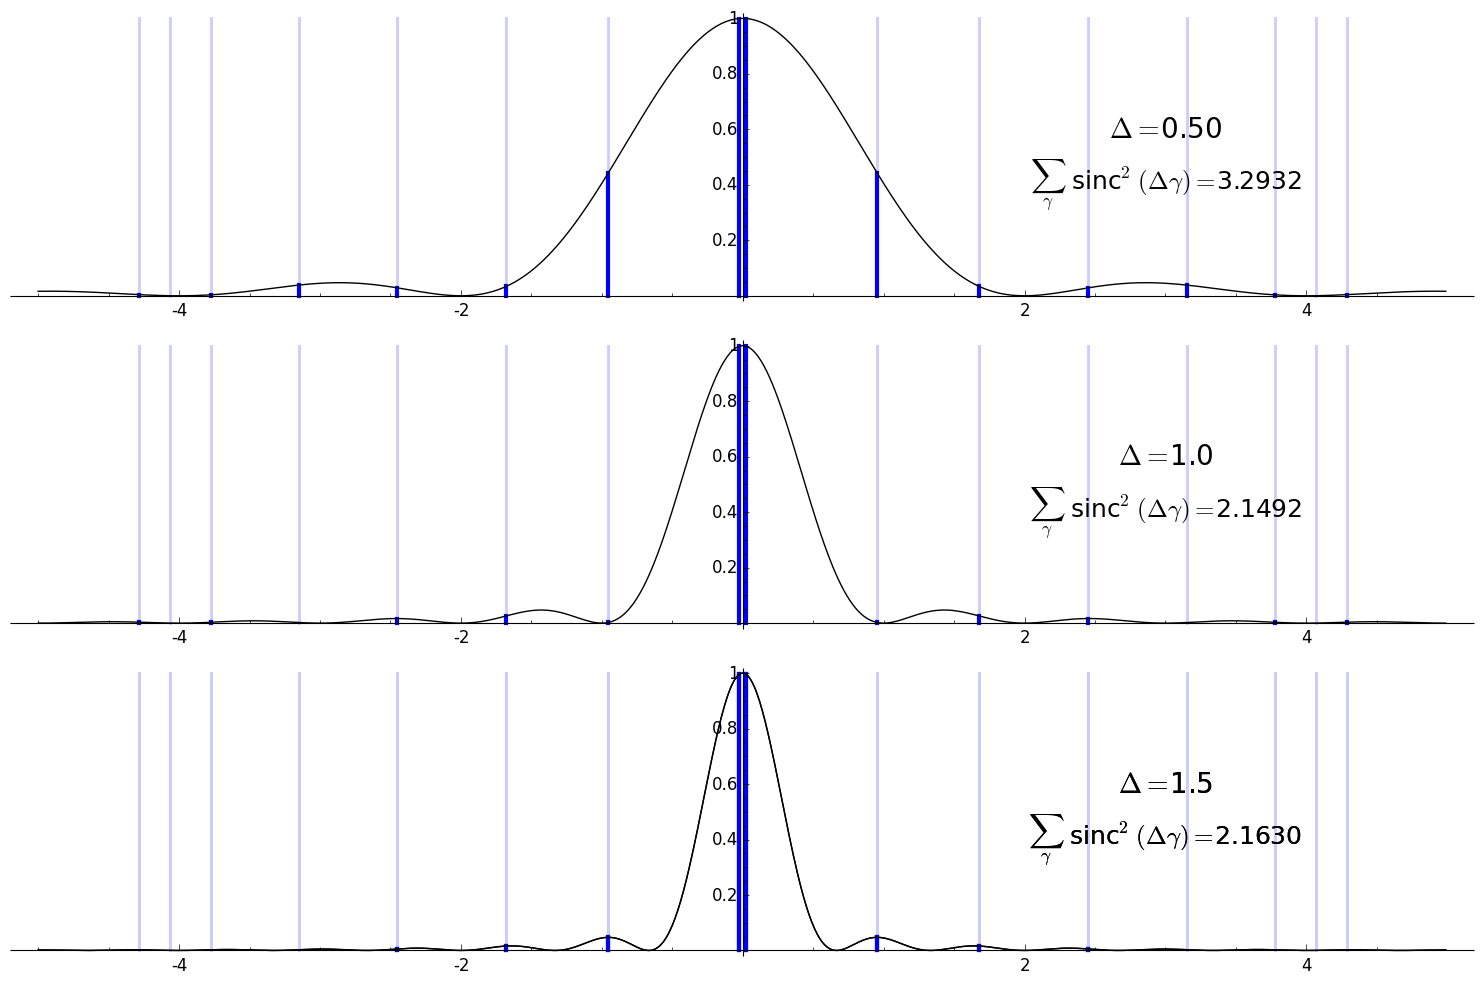
\includegraphics[width=1.0\textwidth]{graphics/256944c1_zero_sum.png}
    \caption{A graphic representation of the $\sinc^2$ sum for the Cremona curve {\tt 256944c1} , a rank 0 curve with conductor $N_E=256944$, for $\Delta = 0.5$, $1.0$ and $1.5$.}
    \label{fig:256944c1_zero_sum}
\end{figure}

However, establishing results regarding the rate of convergence of this sum proves more elusive. Consider the example in Figure \ref{fig:256944c1_zero_sum}: the Cremona curve {\tt 256944c1}, a rank 0 curve, has a pathologically low-lying zero at $\gamma_0 = 0.02560\ldots$. For small values of $\Delta$, it therefore appears that this curve has analytic rank 2, not zero. In fact, only for $\Delta>\sim 2.815$ does the sum evaluate to a value less than 2 (which, after invoking parity, gives us that it is rank 0). This highlights the fact that some curves -- specifically those with low-lying zeros -- require $\Delta$ to be large for the sum to be within, say, 2 of the true rank of the curve. \\

Furthermore, Figure \ref{fig:256944c1_zero_sum} shows that the convergence from above is unfortunately {\it not} even necessarily monotone: as $\Delta$ is increased the small outlying bumps of the sinc$^2$ function can travel over zeros and temporarily increase the value of the sum. \\

Even though this is the case, we should be able to make some sort of a convexity statement regarding the convergence of the sinc$^2$ sum. This should allow us to use point estimates in the rank estimation code to decide which $\Delta$ values to use on a given curve, and in so doing make the code more efficient. We hope to revisit this issue in future, as it has the potential to significantly increase the effectiveness of the rank estimation code.

%%%%%%%%%%%%%%%%%%%%%%%%%%%%%%%%%%%%%%%%%%%%%%%%%%%%%%%
\section{Better bounds on the bite}

Section \ref{sec:bite} discusses at the topic of the bite of an elliptic curve, namely the quantity
\begin{equation}
\beta_E = \sum_{\gamma \ne 0} \frac{1}{\gamma^2}
\end{equation}

It would be useful to have better bounds in either direction for this quantity. In terms of bounding from below, we are reasonably confident that the constant $K(\epsilon)$ in Equation \ref{eqn:bite_lower_bound} can be made explicit in terms of $\epsilon$, given more diligent controlling of the various zero sum-based inequalities. Better yet, it would seem that the bite must grow faster than any multiple of $\log N_E$, and we would like to show that this is the case. It is conceivable that this could also be achieved using the methods detailed in this work. \\

On the other hand, placing an upper bound on the bite is equivalent to bounding the lowest noncentral zero away from the central point. This is a much deeper and more difficult endeavour, equivalent to placing a lower bound on the leading central Taylor coefficient of $\Les$. The latter is done in Chapter \ref{chap:main_theorem}, and in fact a direct corollary of this is that the lowest noncentral zero $\gamma_0$ is bounded below by $(N_E)^{-\alpha}$ for some $\alpha>0$. However, in the leading Taylor coefficient bound a constant introduced from the bound on the real period is never made explicit; while this is good enough to get a polynomial-time rank algorithm out, it {\it isn't} good enough to make the lower bound on $\gamma_0$ explicit. Again, we hope that this issue can be resolved in future work, perhaps by making all constants in bounds on the real period completely explicit.


